\chapter{Esempio di impiego}
\label{app:esempio}
\thispagestyle{empty}

\begin{quotation}
{\footnotesize
\noindent{\emph{Doc: Scusa, la rozzezza di questo modello ma non ho avuto il tempo di farlo in scala e di dipingerlo. \\
Marty: Va bene, va bene.
} }
\begin{flushright}
Ritorno al Futuro, parte III
\end{flushright}
}
\end{quotation}
\vspace{0.5cm}

Mostriamo in questo capitolo il sistema hardware e software utilizzato per testare i concetti, gli algoritmi e le metodologie presentate in questa tesi.

\section{Robot}
Il robot preso in considerazione per i nostri test sperimentali è un quadrotor. Abbiamo utilizzato l'A.R. Drone, prodotto da Parrot. 
Il quadrotor utilizzato è dotato di una telecamera HD con risoluzione $640\times 480$, tuttavia nella tesi sono state utilizzate immagini a $320\times 240$, a 30 frame al secondo.
La qualità delle immagini è scadente, e sono affette da pesanti problemi di refresh.
Il robot possiede anche una unità di misura inerziale economica e un magnetometro.
Inoltre il robot possiede una telecamera inferiore, di risoluzione $320\times 240$, la cui qualità dell'immagine è molto peggiore rispetto alla telecamera frontale, che tuttavia non è stata sfruttata per lo svolgimento di questa tesi.

\'E stato scelto di utilizzare questo quadrotor per alcuni validi motivi:
\begin{itemize}
 \item L'hardware è a basso costo, e il quadrotor si trova in commercio a un prezzo relativamente basso.
 \item Il robot in questione ha 6 gradi di libertà nello spazio, questo rende possibile lo studio di un sistema di localizzazzione e mapping in 3 dimensioni.
 \item Il robot è già integrato con ROS.
\end{itemize}


\section{Hardware e software di controllo}
Per controllare il quadrotor e lanciare l'algoritmo di controllo è stato utilizzato un portatile dotato di processore Intel Core i7-4500U, e 4GB di RAM DDR3.
Il portatile utilizzato si occupava, oltre che di gestire l'algoritmo di controllo, di visualizzare output di debug.
Per il controllo del drone è stato utilizzato il driver \textit{ardrone\_autonomy}, disponibile nei repository di ROS.
Per muovere il quadrotor è stato utilizzato un joystick, integrato con ROS tramite il nodo \textit{joy}, anchesso presente nei repository ufficiali di ROS.
Per impartire comandi dal joystick al quadrotor ci si è avvalsi di un controllore già implementato nel package  \textit{ardrone\_tutorials}, che fornisce anche una finestra che mostra l'immagine presa direttamente dalla telecamera del drone.

\section{Classificatore utilizzato}

Il classificatore utilizzato prende in input rettangoli e cluster.
La struttura del classificatore è data dal seguente file:

\begin{lstlisting}[language=fuzzyClassifier]
CLASS Rectangle HIDDEN
	VARIABLES
		xMin;
		xMax;
		yMin;
		yMax;
		formFactor;
		area;
	END_VARIABLES
END_CLASS

CLASS Cluster HIDDEN
	VARIABLES
		x;
		y;
	END_VARIABLES
END_CLASS

CLASS WhiteBoard extends Rectangle
	area is Big;
	formFactor is Wide;
END_CLASS

CLASS LargeWhiteBoard extends Rectangle
	area is VeryBig;
	formFactor is VeryWide;
END_CLASS

CLASS Cabinet extends Rectangle
	area is Huge;
	formFactor is Medium;
END_CLASS

CLASS CabinetDoor extends Rectangle
	area is VeryBig;
	formFactor is Narrow;
END_CLASS

CLASS PossibleDoor extends Rectangle
	formFactor is VeryNarrow;
	area is VeryBig;
END_CLASS

CLASS Door extends PossibleDoor
	
	CONSTANTS
		height = High;
	END_CONSTANTS
	
	Handle.x is Lateral on(xMin, xMax);
	Handle.y is Centered on(yMin, yMax);

END_CLASS

CLASS Handle extends Cluster	
	x is Lateral on Door(xMin, xMax);
	y is Centered on Door(yMin, yMax);
END_CLASS
\end{lstlisting}

La knowledgebase di riferimento è definita nel modo seguente:

\begin{lstlisting}[language=fuzzyKnowledgebase]
FUZZIFY_CLASS Rectangle
	FUZZIFY formFactor
		VeryNarrow := tra(2600, 2700, 2900, 3000);
		Narrow := tra(1900, 2000, 2600, 2700);
		Medium := tra(900, 1000, 1100, 1500); 
		Wide := tra(850, 900, 920, 970);
		VeryWide := tra(700, 800, 850, 900);
	END_FUZZIFY
	
	FUZZIFY area
		Big := tor(7000, 7500);
		VeryBig := tor(9000, 10000);
		Huge := tor(20000, 25000);
	END_FUZZIFY
END_FUZZIFY_CLASS

FUZZIFY_CLASS Cabinet
END_FUZZIFY_CLASS

FUZZIFY_CLASS CabinetDoor
END_FUZZIFY_CLASS

FUZZIFY_CLASS WhiteBoard
END_FUZZIFY_CLASS

FUZZIFY_CLASS LargeWhiteBoard
END_FUZZIFY_CLASS

FUZZIFY_CLASS PossibleDoor
END_FUZZIFY_CLASS

FUZZIFY_CLASS Door

	FUZZIFY_PREDICATE ?x
		Lateral := (?x is Left) or (?x is Right);
		Centered := (?x is Centered);
		
		FUZZIFY ?x
			Left := tol(20, 30);
			Centered := tra(40, 50, 55, 60);
			Right := tor(70, 80);
		END_FUZZIFY
		
	END_FUZZIFY_PREDICATE	
	
END_FUZZIFY_CLASS

FUZZIFY_CLASS Cluster
END_FUZZIFY_CLASS


FUZZIFY_CLASS Handle

	FUZZIFY_PREDICATE ?x
		Lateral := (?x is Left) or (?x is Right);
		Centered := (?x is Centered);
		
		FUZZIFY ?x
			Left :=  tol(30, 40);
			Centered :=  tra(30, 40, 60, 80);
			Right :=  tor(60, 80);
		END_FUZZIFY
		
	END_FUZZIFY_PREDICATE	
	
END_FUZZIFY_CLASS
\end{lstlisting}

Il grafo delle dipendenze generato da questo classificatore è mostrato in \autoref{fig:grafo-dipendenze} mentre il grafo di reasoning in \autoref{fig:grafo-reasoning}. Nel grafo delle dipendenze le frecce continue rappresentano relazioni di sottoclasse, mentre le frecce tratteggiate rappresentano una relazione di dipendenza.

\begin{figure}[ht]
  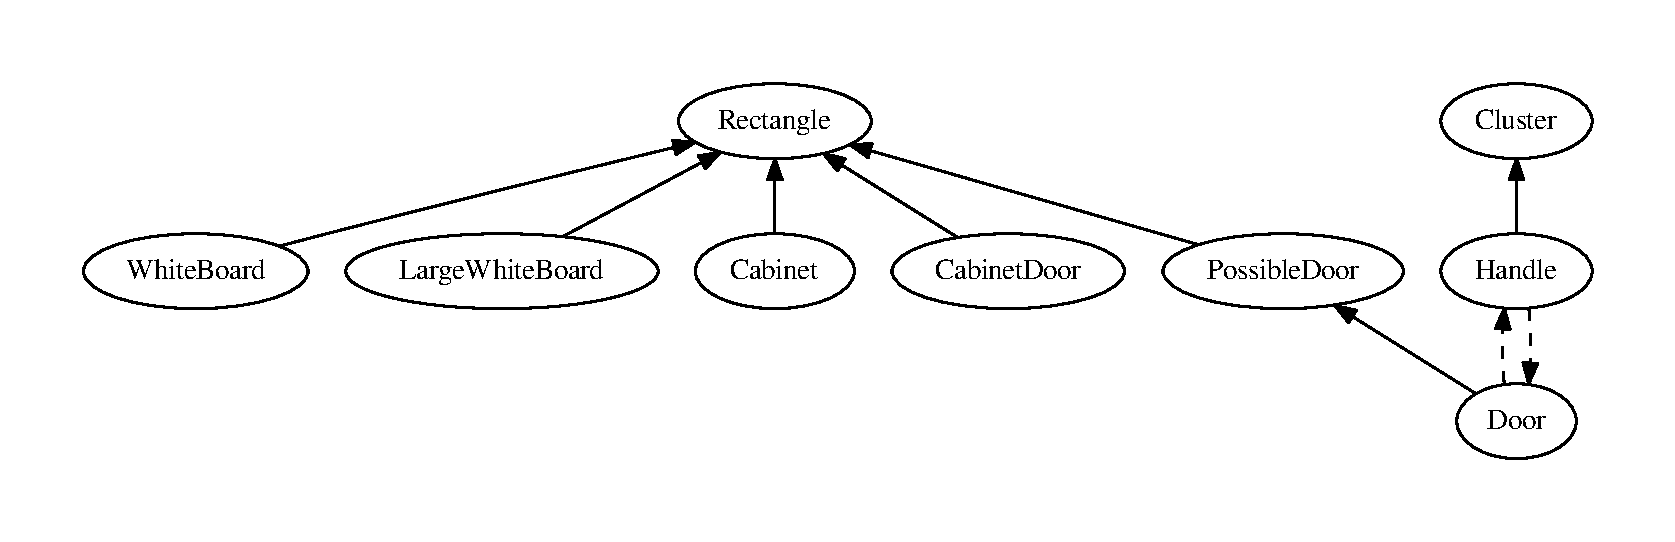
\includegraphics[width=\textwidth]{diagrammi/classifier}
  \caption{Grafo delle dipendenze}
  \label{fig:grafo-dipendenze}
\end{figure}

\begin{figure}[ht]
  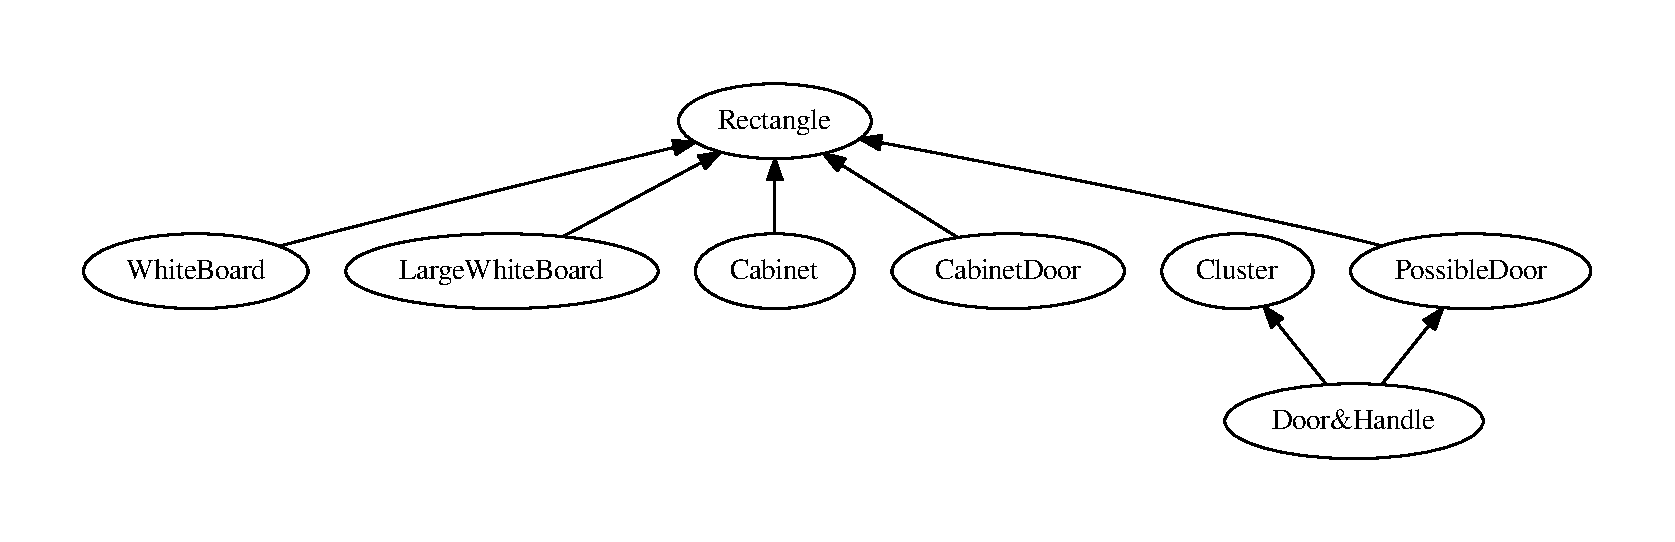
\includegraphics[width=\textwidth]{diagrammi/reasoning}
  \caption{Grafo di reasoning}
  \label{fig:grafo-reasoning}
\end{figure}
